\documentclass[../main.tex]{subfiles}

\begin{document}
\section{Introduction to astrophysics and satellite tracking}
\subsection{The two body problem}\label{sec:twoBody}
\subsubsection{Trajectory equation}
We are interested in understanding the dynamics of a spacecraft in orbit around the Earth. These dynamics are governed by Newton's second law of motion, which assuming that both the Earth and the spacecraft are point masses (see \cref{sec:force} for a more realistic model), can be written as
\begin{equation}
  \label{eq:Newton}
  \ddot{\vf{r}}=-\frac{GM_{\oplus}}{r^2}\vf{e}_r
\end{equation}
where $\vf{r}$ is the position vector (also called \emph{radius vector}) of the spacecraft with respect to the Earth, $r:=\norm{\vf{r}}$, $\vf{e}_r=\frac{\vf{r}}{r}$ is the unit vector in the direction of $\vf{r}$, $M_{\oplus}\simeq 5.972\times 10^{24}\ \kg$ is the mass of the Earth, and $G\simeq 6.674\times 10^{-11}\ \m^3\cdot \kg^{-1}\cdot\s^{-2}$ is the gravitational constant. Note that the minus sign is due to the fact that the gravitational force is attractive, i.e. pointing towards the Earth.
Here and along the document the notation $\ddot{\vf{r}}$ means that the derivative is taken with respect to time.
Cross-multiplying \cref{eq:Newton} by $\vf{r}$, we obtain
\begin{equation}
  \dv{(\vf{r}\times \dot{\vf{r}})}{t}=\dot{\vf{r}}\times \dot{\vf{r}}+\vf{r}\times\ddot{\vf{r}}=-\frac{GM_{\oplus}}{r^3}(\vf{r}\times \vf{r})=0
\end{equation}
Hence $\vf{r}\times \dot{\vf{r}}=:\vf{h}$ is constant. The physical intuition behind this is that the motion of the spacecraft around the Earth is confined to a plane, which is called the \emph{orbital plane} because the position $\vf{r}$ and velocity $\vf{r}$ are always perpendicular to $\vf{h}$, which is the normal vector to the orbital planes and it relates to the \emph{angular momentum} of the spacecraft.

We are interested now in what kind of curves may be described by a body orbiting the other one. That is, we want somehow isolate $\vf{r}$ (or $r$) from \cref{eq:Newton}. In order to simplify the notation we will denote $\mu:=GM_{\oplus}$.
\begin{proposition}[Kepler's first law]
  \label{prop:two-body}
  The motion of a body orbiting another one is described by a conic. Hence it can be expressed in the form:
  \begin{equation}
    \label{eq:two-body}
    r(t)=\frac{p}{1+e\cos (\nu(t))}
  \end{equation}
  for some parameters $p$ and $e$.
\end{proposition}
\begin{proof}
  Cross-multiplying \cref{eq:Newton} by $\vf{h}$ we obtain
  \begin{equation}\label{eq:rtimesh}
    \dv{(\dot{\vf{r}}\times\vf{h})}{t}=\ddot{\vf{r}}\times\vf{h}=-\frac{\mu}{r^3}\vf{r}\times\vf{h}=-\frac{\mu}{r^3}\vf{r}\times(\vf{r}\times \dot{\vf{r}})=-\frac{\mu}{r^3}[(\vf{r}\cdot{\vf{r}})\dot{\vf{r}}-(\vf{r}\cdot\dot{\vf{r}})\vf{r}]
  \end{equation}
  where we have used \cref{prop:triplecross}. Now note that:
  \begin{equation}
    \dv{}{t}\left(\frac{\vf{r}}{r}\right)=\frac{\dot{\vf{r}}}{r}-\frac{\dot{r}}{r^2}\vf{r}= \frac{1}{r^3}[(\vf{r}\cdot{\vf{r}})\dot{\vf{r}}-(\vf{r}\cdot\dot{\vf{r}})\vf{r}]
  \end{equation}
  because $2r\dot{r}=\dv{(r^2)}{t}=\frac{(\vf{r}\cdot\vf{r})}{t}=2\vf{r}\cdot\dot{\vf{r}}$\footnote{Bear in mind that in general $\dot{r}\ne\norm{\dot{\vf{r}}}$. Indeed, if $\beta$ denotes the angle between $\vf{r}$ and $\dot{\vf{r}}$ we have that $\dot{r}=\norm{\dot{\vf{r}}}\cos\beta$. In particular $\dot{r}$ may be negative.}. Thus:
  \begin{equation}
    \dv{(\dot{\vf{r}}\times\vf{h})}{t}=\mu \dv{}{t}\left(\frac{\vf{r}}{r}\right)
  \end{equation}
  Integrating with respect to the time yields
  \begin{equation}\label{eq:rdottimesh}
    \dot{\vf{r}}\times \vf{h}=\frac{\mu}{r}\vf{r}+\vf{B}
  \end{equation}
  where $\vf{B}\in\RR^3$ is the constant of integration. Observe that since $\dot{\vf{r}}\times\vf{h}$ is perpendicular to $\vf{h}$, it lies in the orbital plane and so does $\vf{r}$. Hence, $\vf{B}$ lies on the orbital plane. Now dot-multiplying this last equation by $\vf{r}$ and using that $\vf{u}\cdot(\vf{v}\times\vf{w})=(\vf{u}\times\vf{v})\cdot\vf{w}$ $\forall\vf{u},\vf{v},\vf{w}\in\RR^3$ we obtain
  \begin{equation}
    h^2=\vf{h}\cdot\vf{h}=(\vf{r}\times\dot{\vf{r}})\cdot\vf{h}=\vf{r}\cdot(\dot{\vf{r}}\times\vf{h})=\frac{\mu}{r}\vf{r}\cdot\vf{r}+\vf{r}\cdot\vf{B}=\mu r+rB\cos\nu
  \end{equation}
  where $h:=\norm{\vf{h}}$, $B:=\norm{\vf{B}}$ and $\nu$ denotes the angle between $\vf{r}$ and $\vf{B}$. Rearranging the terms we obtain finally the equation of a conic
  \begin{equation}\label{eq:r_conic}
    r=\frac{h^2/\mu}{1+(B/\mu)\cos(\nu)}
  \end{equation}
  with $p:=h^2/\mu$ and $e:=B/\mu$.
\end{proof}
Among the range of values that can $r$ take, we are particularly interested in the minimum and maximum values, $r_\mathrm{min}$ and $r_\mathrm{max}$, that can be attained. Is easy to see that these are given by
\begin{equation}
  r_\mathrm{min}=\frac{p}{1+e}\qquad\text{and}\qquad r_\mathrm{max}=
  \begin{cases}
    \displaystyle\frac{p}{1-e} & e<1     \\
    \infty                     & e\geq 1
  \end{cases}
\end{equation}
The points on the orbit of such distances are attained are called \emph{apoapsis} and \emph{periapsis} respectively. The line connecting both points is called \emph{line of apsides}, and the half of the distance between them is the \emph{semi-major axis} and is denoted by $a$:
\begin{equation}\label{eq:semi-major_axis}
  a:=\frac{r_\mathrm{max}+r_\mathrm{min}}{2}=
  \begin{cases}
    \displaystyle\frac{p}{1-e^2} & e<1     \\
    \infty                       & e\geq 1
  \end{cases}=
  \begin{cases}
    \displaystyle\frac{h^2}{\mu(1-e^2)} & e<1     \\
    \infty                              & e\geq 1
  \end{cases}
\end{equation}
because we have considered the reference frame of \cref{fig:conics_cartesian} and so the line of apsides crosses the origin. Finally the angle $\nu$ is called \emph{true anomaly}. Note that at $\vf{r}_\mathrm{min}$, we have $\nu=0$ and so $\vf{r}\parallel\vf{B}$. Hence $\vf{B}$ points towards the periapsis of the orbit.
\begin{definition}
  Let $\vf{r}(t)$, $\vf{r}(t+k)$ be the positions of the small body at times $t$, $t+k$ respectively. Let $A(t)$ be the area swept by the radius vector $\vf{r}(t)$ in the time interval $[0,t]$. We define the \emph{areal velocity} as $\dv{A(t)}{t}$.
\end{definition}
\begin{proposition}[Kepler's second law]
  The areal velocity remains constant.
\end{proposition}
\begin{proof}
  Recall that the area of a parallelogram generated by two vectors $\vf{u},\vf{v}\in\RR^3$ is given by $\norm{\vf{u}\times\vf{v}}$. Thus, approximating the area $A$ by half of the parallelogram generated by $\vf{r}(t)$ and ${\vf{r}}(t+k)$ we obtain
  \begin{multline}\label{eq:areal_velocity}
    \dv{A(t)}{t}=\lim_{k\to 0}\frac{A(t+k)-A(t)}{k}=\lim_{k\to 0}\frac{\norm{\vf{r}(t)\times\vf{r}(t+k)}}{2k}=\lim_{h\to 0}\frac{\norm{\vf{r}(t)\times(\vf{r}(t+k)-\vf{r}(t))}}{2k}=\\
    =\frac{\norm{\vf{r}(t)\times\dot{\vf{r}}(t)}}{2}=\frac{h}{2}
  \end{multline}
  where the penultimate equality is because the cross product is continuous and linear.
\end{proof}
Finally we will need the following equation which relates the velocity of the satellite with the distance to the central of the Earth.
\begin{proposition}
  We have that (\cite{montenbruck}):
  \begin{equation}\label{eq:visviva}
    v^2=\mu\left(\frac{2}{r}-\frac{1}{a}\right)
  \end{equation}
  where $v:=\norm{\dot{\vf{r}}}$.
\end{proposition}
\begin{proof}
  Using \cref{eq:rdottimesh} we have that $\vf{h}\times\vf{r}=(\vf{r}\cdot\dot{\vf{r}})\vf{r}-(\vf{r}\cdot{\vf{r}})\dot{\vf{r}}$ and so:
  \begin{equation}
    \norm{\vf{h}\times\dot{\vf{r}}}^2=\frac{\mu^2}{r^2}\vf{r}\cdot\vf{r}+2\frac{\mu}{r}\vf{r}\cdot\vf{B}+\vf{B} \cdot \vf{B}=\mu^2(1+2 e\cos\nu + e^2)=\mu^2(2(1+ e\cos\nu) -(1- e^2))
  \end{equation}
  where we have used that $e\mu=B$ (see \cref{eq:r_conic}). Now using \cref{eq:r_conic,eq:semi-major_axis} we obtain that
  \begin{equation}
    2(1+ e\cos\nu) -(1- e^2)=2\frac{p}{r}-\frac{h^2}{\mu a}=2\frac{h^2}{r\mu}-\frac{h^2}{\mu a}
  \end{equation}
  Since $\vf{h}\perp\dot{\vf{r}}$, $\norm{\vf{h}\times\dot{\vf{r}}}=hv$ and so:
  \begin{equation}
    v^2=\mu\left(\frac{2}{r}-\frac{1}{a}\right)
  \end{equation}
\end{proof}
From now one we will suppose that the orbits are ellipses, which is the main case of interest.
\subsubsection{Kepler's equation}
So far we have been able to describe the geometry of motion of a body orbiting another one. However, we have not been concerned about the specific position of the body as a function of time. That is how to obtain $\nu(t)$ at each instant of time. In order to do this, we may think the area $A$ as a function of $\nu$, that measures the area swept by the radio vector from an initial instant $\nu_0$. Thus, from differential calculus we know that:
\begin{equation}
  A(\nu)=\int_{\nu_0}^{\nu}\int_{0}^{r(\theta)}r\dd{r}\dd{\theta}=\int_{\nu_0}^{\nu}\frac{r(\theta)^2}{2}\dd{\theta}\implies\dv{A}{\nu}=\frac{r^2}{2}
\end{equation}
And using the chain rule and \cref{eq:areal_velocity} we obtain that:
\begin{equation}\label{eq:areal_velocity_nu}
  \frac{h}{2}=\dv{A}{t}=\dv{A}{\nu}\dv{\nu}{t}=\frac{r^2}{2}\dot\nu
\end{equation}
So from \cref{eq:r_conic,eq:areal_velocity_nu} we get the following differential equation that must satisfy $\nu$:
\begin{equation}
  \dot\nu=\frac{h}{r^2}=\frac{h}{p^2}{(1+e\cos\nu)}^2
\end{equation}
which, when integrated with respect to the time, lead us to an elliptic integral. Our goal in this section is to find an easier way to compute exact position of the satellite ate each instant of time. This will lead us to the so-called \emph{Kepler's equation}. For this purpose we are forced to introduce a new parameter, $E$, called \emph{eccentric anomaly}. It is defined as the angle between the line of apsides and the line passing through the center of the ellipse and the point at the circle which is just above the position of the satellite (see \cref{fig:kepler_eq} for a better understanding).
\begin{figure}[ht]
  \centering
  \includegraphics[width=0.5\textwidth]{Images/kepler_eq.pdf}
  \caption{Ellipse orbit of the satellite together with an auxiliary circle of radius $a$ needed to define the eccentric anomaly.}
  \label{fig:kepler_eq}
\end{figure}

Clearly the position of the satellite is determined by $x=r\cos\nu$, $y=r\sin\nu$. But we would like to find an expression of $x$ and $y$ in terms of $E$ rather than $\nu$. To do this note that $a\cos E=ae+x$, so:
\begin{equation}\label{eq:eccentricX}
  x=a(\cos E-e)
\end{equation}
And so we can get an expression of $r$ in terms of $E$ by solving the equation:
\begin{equation}\label{eq:eccentricr}
  r=\frac{p}{1+e\cos \nu}=\frac{a(1-e^2)}{1+e\frac{x}{r}}=\frac{ra(1-e^2)}{r+ae(\cos E-e)}\implies r= a(1-e\cos E)
\end{equation}
Finally from \cref{eq:eccentricX,eq:eccentricr} we get:
\begin{equation}
  y^2=r^2-x^2=a^2(1-e^2){(\sin E)}^2\implies y=a\sqrt{1-e^2}\sin E
\end{equation}
Expressing now the areal velocity $h$ as a function of $E$ we have:
\begin{align}
  h & =x\dot{y}-y\dot{x}                                                           \\
    & =a^2(\cos E-e)\sqrt{1-e^2}(\cos E)\dot{E}+a^2{(\sin E)}^2\dot{E}\sqrt{1-e^2} \\
    & =a^2\sqrt{1-e^2}\dot{E}(1-e\cos E)
\end{align}
From \cref{eq:semi-major_axis} we know that $h=\sqrt{\mu a(1-e^2)}$. Thus substituting this in the latter equation we deduce that $E$ must satisfy the following differential equation:
\begin{equation}
  \dot{E}(1-e\cos E)=\sqrt{\frac{\mu}{a^3}}=:n
\end{equation}
where $n$ is called the \emph{mean motion}. Integrating this equation with respect to time yield the \emph{Kepler's equation}:
\begin{equation}
  E(t)-e\sin E(t)=n(t-t_0)
\end{equation}
where $t_0$ is the time at which $E$ vanishes. Using the reference frame of \cref{fig:kepler_eq} this corresponds at the time at which the satellite is at the perigee. The value $M:=n(t-t_0)$ is called \emph{mean anomaly}.

Kepler's equation is the key to solve the problem of finding the position of the satellite at each instant of time. Later on we will discuss techniques to solve this equation for $E$ knowing $e$ and $M$.

\subsection{Time and reference systems}
\subsubsection{Time measurement}
As human beings, we are naturally interested in how time passes and so the correct measure of it becomes an essential necessity for us. As it is the sun that governs our daily activity, it is natural to define time from it.

An \emph{apparent solar day} is defined to be the time between two successive transits of the sun across our local meridian. One should note that the Earth has to rotate on itself slightly more than one revolution in order to complete one solar day. The \emph{apparent siderial day} is defined as the time it take to the Earth to complete a rotation relative to very far away stars (see \cref{fig:siderial} for a beter understanding). The non-circular orbit of the Earth around the sun causes some days to be shorter than others due to Kepler's second law. So the introduction of a \emph{mean solar day} and \emph{mean siderial day} are necessary, which are defined as if the Earth was in a circular orbit of the same period as the true one.

\begin{definition}
  The \emph{Greenwich mean time} (GMT) or \emph{Universal time} (UT or UT1 for disambiguation\footnote{There are other times also referred as \emph{universal}, such as UT1R or UT12 but we will not talk about them in the document.}) is defined as the mean solar time at the Greenwich meridian. The \emph{Greenwich mean siderial time} (GMST) is a representation of the \emph{mean siderial day} and it is defined as the angle between the Greenwich meridian and th emean vernal equinox of date. In a similar way, the \emph{Greenwich aparent siderial time} (GAST) is a representation of the \emph{siderial day} and it is defined as the angle between the Greenwich meridian and the true vernal equinox of date.
\end{definition}

\begin{figure}[ht]
  \centering
  \includegraphics[width=0.5\textwidth]{Images/siderial.pdf}
  \caption{Solar and siderial days (not to scale)}
  \label{fig:siderial}
\end{figure}

In the middle of the 20th century, \emph{Ephemerides time} (ET) was introduced to cope with the irregularities of the Earth's rotation (see POLAR MOTION). This time was defined from historical observations of planets in a Newtonian physics isolating the time from the equations. At the end of the century, the \emph{Terrestrial time} (TT) succeed ET in a relativistic frame. In the meantime, in 1955 \emph{atomic time} (TAI, from French \emph{Temps Athomique International}) was adopted as the SI unit of second. The origin was adopted such that the TAI matches UT at the 00:00:00 UT of January 1st, 1958, yielding the relation
\begin{equation}
  \text{TT}=\text{ET}= \text{TAI} + 32.184\,\mathrm{s}
\end{equation}

Finally, our everyday clock is based on the \emph{Coordinated Universal Time} (UTC). It is defined to be as uniform as the TAI but always kept closer than 0.9 seconds to the UT1 (see GRAPH-TIME). Scientists achieve this by introducing a \emph{leap second} which is an extra second added to UTC at irregular intervals. The last leap second was added on June 30th, 2012. The next one is expected to be added on December 31st, 2016.
\cref{fig:graph_time} summarizes all the time systems introduced in the document.

\begin{figure}[htbp]
  \centering
  \begin{minipage}[t]{0.45\textwidth}
    \centering
    \includegraphics[width=\textwidth]{Images/graph_time.pdf}
    \caption{Evolution of times TT, UT1 and UTC in comparison with TAI. \cite{iersDeltaT}}
    \label{fig:graph_time}
  \end{minipage}
  \hfill
  \begin{minipage}[ht]{0.45\textwidth}
    \centering
    \includegraphics[width=0.9\textwidth]{Images/leap_second.pdf}
    \caption{Leap second introduced to the UTC time at the end of the December 1998. \cite{iersbulletinC}}
    \label{fig:leapsecond}
  \end{minipage}
\end{figure}
The folowing conversions between time systems are useful:
\begin{align*}
  \text{GMST} & =24110.54841+8640184.812866{T_\text{UT1}}+0.093104{(T_\text{UT1})}^2-6.2\cdot 10^{-6}{(T_\text{UT1})}^3 \\
  \text{UT1}  & =\text{TT}-\Delta T                                                                                     \\
  \text{TT}   & =\text{TAI}-32.184                                                                                      \\
  \text{TAI}  & =\text{UTC}+\delta(\text{TAI})
\end{align*}
where $ T=\frac{\text{JD}(\text{UT1})-2451545}{36525}$ is the number of Julian centuries since the epoch J2000.0, $\Delta T$ is the difference between the TT and UT1, $\delta(\text{TAI})$ is a piecewise constant function that counts the number of leap seconds introduced since 1972 (when they were introduced for the first time). All the numbers have units of second. Note that since the rotation of the Earth cannot be predicted accurately, $\Delta T$ can only be determined retrospectively, and is given by the \emph{International Earth Rotation and Reference Systems Service} (IERS).
\subsubsection{Reference systems}
Newton's second law in only valid when applied to an \emph{inertial reference frame}, that is, a frame of reference that is not undergoing any acceleration. In practise, however, almost any frame of reference is not inertial. So in this chapter we will describe an almost-inertial frame of reference which will be used to integrate Newton's second law. On the other hand, since the earth is not a perfect sphere and there are zones which higher mass density than others, and therefore with higher gravitational field (see SPHERICAL-HARMONICS), we would need the longitude and latitude of the satellite with respect to the Earth at each time of integration. Hence, a Earth-centered system will be needed too.

The first reference frame we must consider is the \emph{celestial}one. On basis of the study of the solar system a natural origin for this frame is the center of mass of the solar system. In order to define the $x$-, $y$-, and $z$-axes, we will need the following definitions.
\begin{definition}
  We define the \emph{celestial equator} as the plane on $\RR^3$ that contains the Earth equator. We define the \emph{celestial ecliptic} as the plane on $\RR^3$ that contains the ecliptic, that is, the orbit of the Earth around the sun. In order to simplify the language, we will call them \emph{equator} and \emph{ecliptic} respectively.
\end{definition}
\begin{definition}
  We define the \emph{celestial sphere} as an abstract sphere of infiniteradius concentric with the Earth. All the celestial objects are thus, projected naturally on the celestial sphere, identifying them with two coordinates (longitude and latitude) (see \cref{fig:precession_matrix} for a better understanding).
\end{definition}
\begin{definition}
  Consider the line $\ell$ of intersection between the celestial equator and the celestial ecliptic. We define the \emph{vernal equinox} as the point $\Upsilon$ on the ecliptic that lies on the line $\ell$ and is such that the Earth is crossing the celestial equator from south to north.
\end{definition}
From here, we can define the $x$-axis as the line $\ell$ and pointing to the vernal equinox, the $z$-axis perpendicular to the celestial equator and the $y$-axis chosen such that the triplet $(x,y,z)$ is a right-handed system.

However, due to the presence of other solar system planets (and other smaller perturbations), the orbital plane of the Earth is not fixed in space, but is subjected to a small variation called \emph{planetary precession}. Moreover, the gravitational attraction of the Sun and Moon on the Earth's equator cause Earth's axis of rotation to precess in a similar way to the action of a spinning top with a period of about 26000 years \cite{montenbruck}. This motion is called \emph{lunisolar precession}. On the other hand, smaller pertubations in amplitude ($<18.6$ years \cite{wiki:eci}) with shorter period superposed with the precessional motion creates a motion called \emph{nutation}. When this latter oscillations are averaged out, the Earth's axis of rotation, the ecliptic, and the equator are referred to \emph{mean} values, rather than \emph{true} values.

In view of this time-dependent orientation of both the ecliptic and the equator, the standard-reference frame chosen is based on the mean equator, mean ecliptic and mean equinox of some fixed time, the beginning of the year 2000, namely at 12:00 TT on 1 January 2000, the so-called \emph{J2000 epoch}.
\begin{definition}[J2000 frame of reference]
  We define the \emph{J2000 frame of reference} as the frame of reference whose $x$-axis is the intersection of the mean celestial equator and the mean celestial ecliptic pointing at the mean vernal equinox, the $z$-axis is perpendicular to the mean ecliptic plane and the $y$-axis is chosen such that the triplet $(x,y,z)$ is a right-handed system. The origin of this system is chosen to be at the center of mass of the solar system.
\end{definition}

Let's move on now to study an Earth-fixed reference frame.
\begin{definition}
  We define the \emph{prime meridian} or \emph{zero meridian} is the meridian that passes through the Royal Observatory in Greenwich, England, and is the reference meridian for longitude measurements.
\end{definition}
\begin{definition}[Earth-fixed frame of reference]
  We define the \emph{Earth-fixed frame of reference} at time $t$ as the frame of reference whose $x$-axis is pointing to the prime meridian, the $z$-axis is perpendicular to the Earth equator at time $t$ and the $y$-axis is chosen such that the triplet $(x,y,z)$ is a right-handed system. The origin of this system is chosen to be at the center of mass of the Earth.
\end{definition}
\subsubsection{Conversion between reference systems}
As we noted in the previous section the angle $\varepsilon$ between the celestial equator and celestial ecliptic planes is not constant due to the planetary precession.

We would like to transform the position of the satellite from the J2000 frame of reference to the Earth-fixed frame of reference and vice versa. This rotation transformation is given by a product of 4 rotations:
\begin{itemize}
  \item The precession matrix $\vf{P}$,
  \item the nutation matrix $\vf{N}$,
  \item the Earth rotation matrix $\vf\Theta$,
  \item and the polar motion matrix $\vf\Pi$.
\end{itemize}
These matrix are such that:
\begin{equation}
  \vf{r}_\mathrm{EF}(t)=\vf\Pi(t)\vf\Theta(t)\vf{N}(t)\vf{P}(t)\vf{r}_{J2000}(t)
\end{equation}
where $\vf{r}_\mathrm{EF}(t)$ is the position vector of the satellite in the Earth-fixed frame of reference at time $t$ and $\vf{r}_{J2000}(t)$ is the position vector of the satellite in the J2000 frame of reference at time $t$. From here on, we will omit the evaluation on the time $t$ for the sake of simplify the lecture.

The precession matrix is responsible for \emph{eliminating} all the movement due to the planetary and lunisolar precession. Thus, $\vf{P}$ transforms the mean equator and mean equinox at time J2000 to the respective values at time $t$. With the help of \cref{fig:precession_matrix} it's not easy to see that this transformation is given by:
\begin{equation}
  \vf{P}=\vf{R}_z(-90-z)\vf{R}_x(\theta)\vf{R}_z(90-\zeta)
\end{equation}
which with a bit of algebra can be simplified to:
\begin{equation}
  \vf{P}=\vf{R}_z(-z)\vf{R}_y(\theta)\vf{R}_z(-\zeta)
\end{equation}
Recall that the fundamental rotation matrices $\vf{R}_x(\theta)$, $\vf{R}_y(\theta)$ and $\vf{R}_z(\theta)$ are with respect to the axis of the J2000 frame and they are given by:
\begin{equation}
  \vf{R}_x(\varphi)=\begin{pmatrix}
    1 & 0            & 0           \\
    0 & \cos\varphi  & \sin\varphi \\
    0 & -\sin\varphi & \cos\varphi
  \end{pmatrix}\;\;\;
  \vf{R}_y(\varphi)=\begin{pmatrix}
    \cos\varphi & 0 & -\sin\varphi \\
    0           & 1 & 0            \\
    \sin\varphi & 0 & \cos\varphi
  \end{pmatrix}\;\;\;
  \vf{R}_z(\varphi)=\begin{pmatrix}
    \cos\varphi  & \sin\varphi & 0 \\
    -\sin\varphi & \cos\varphi & 0 \\
    0            & 0           & 1
  \end{pmatrix}
\end{equation}
where we have used the convention of signs given by \cite{goldstein}.
\begin{figure}[htbp]
  \centering
  \begin{minipage}[t]{0.45\textwidth}
    \centering
    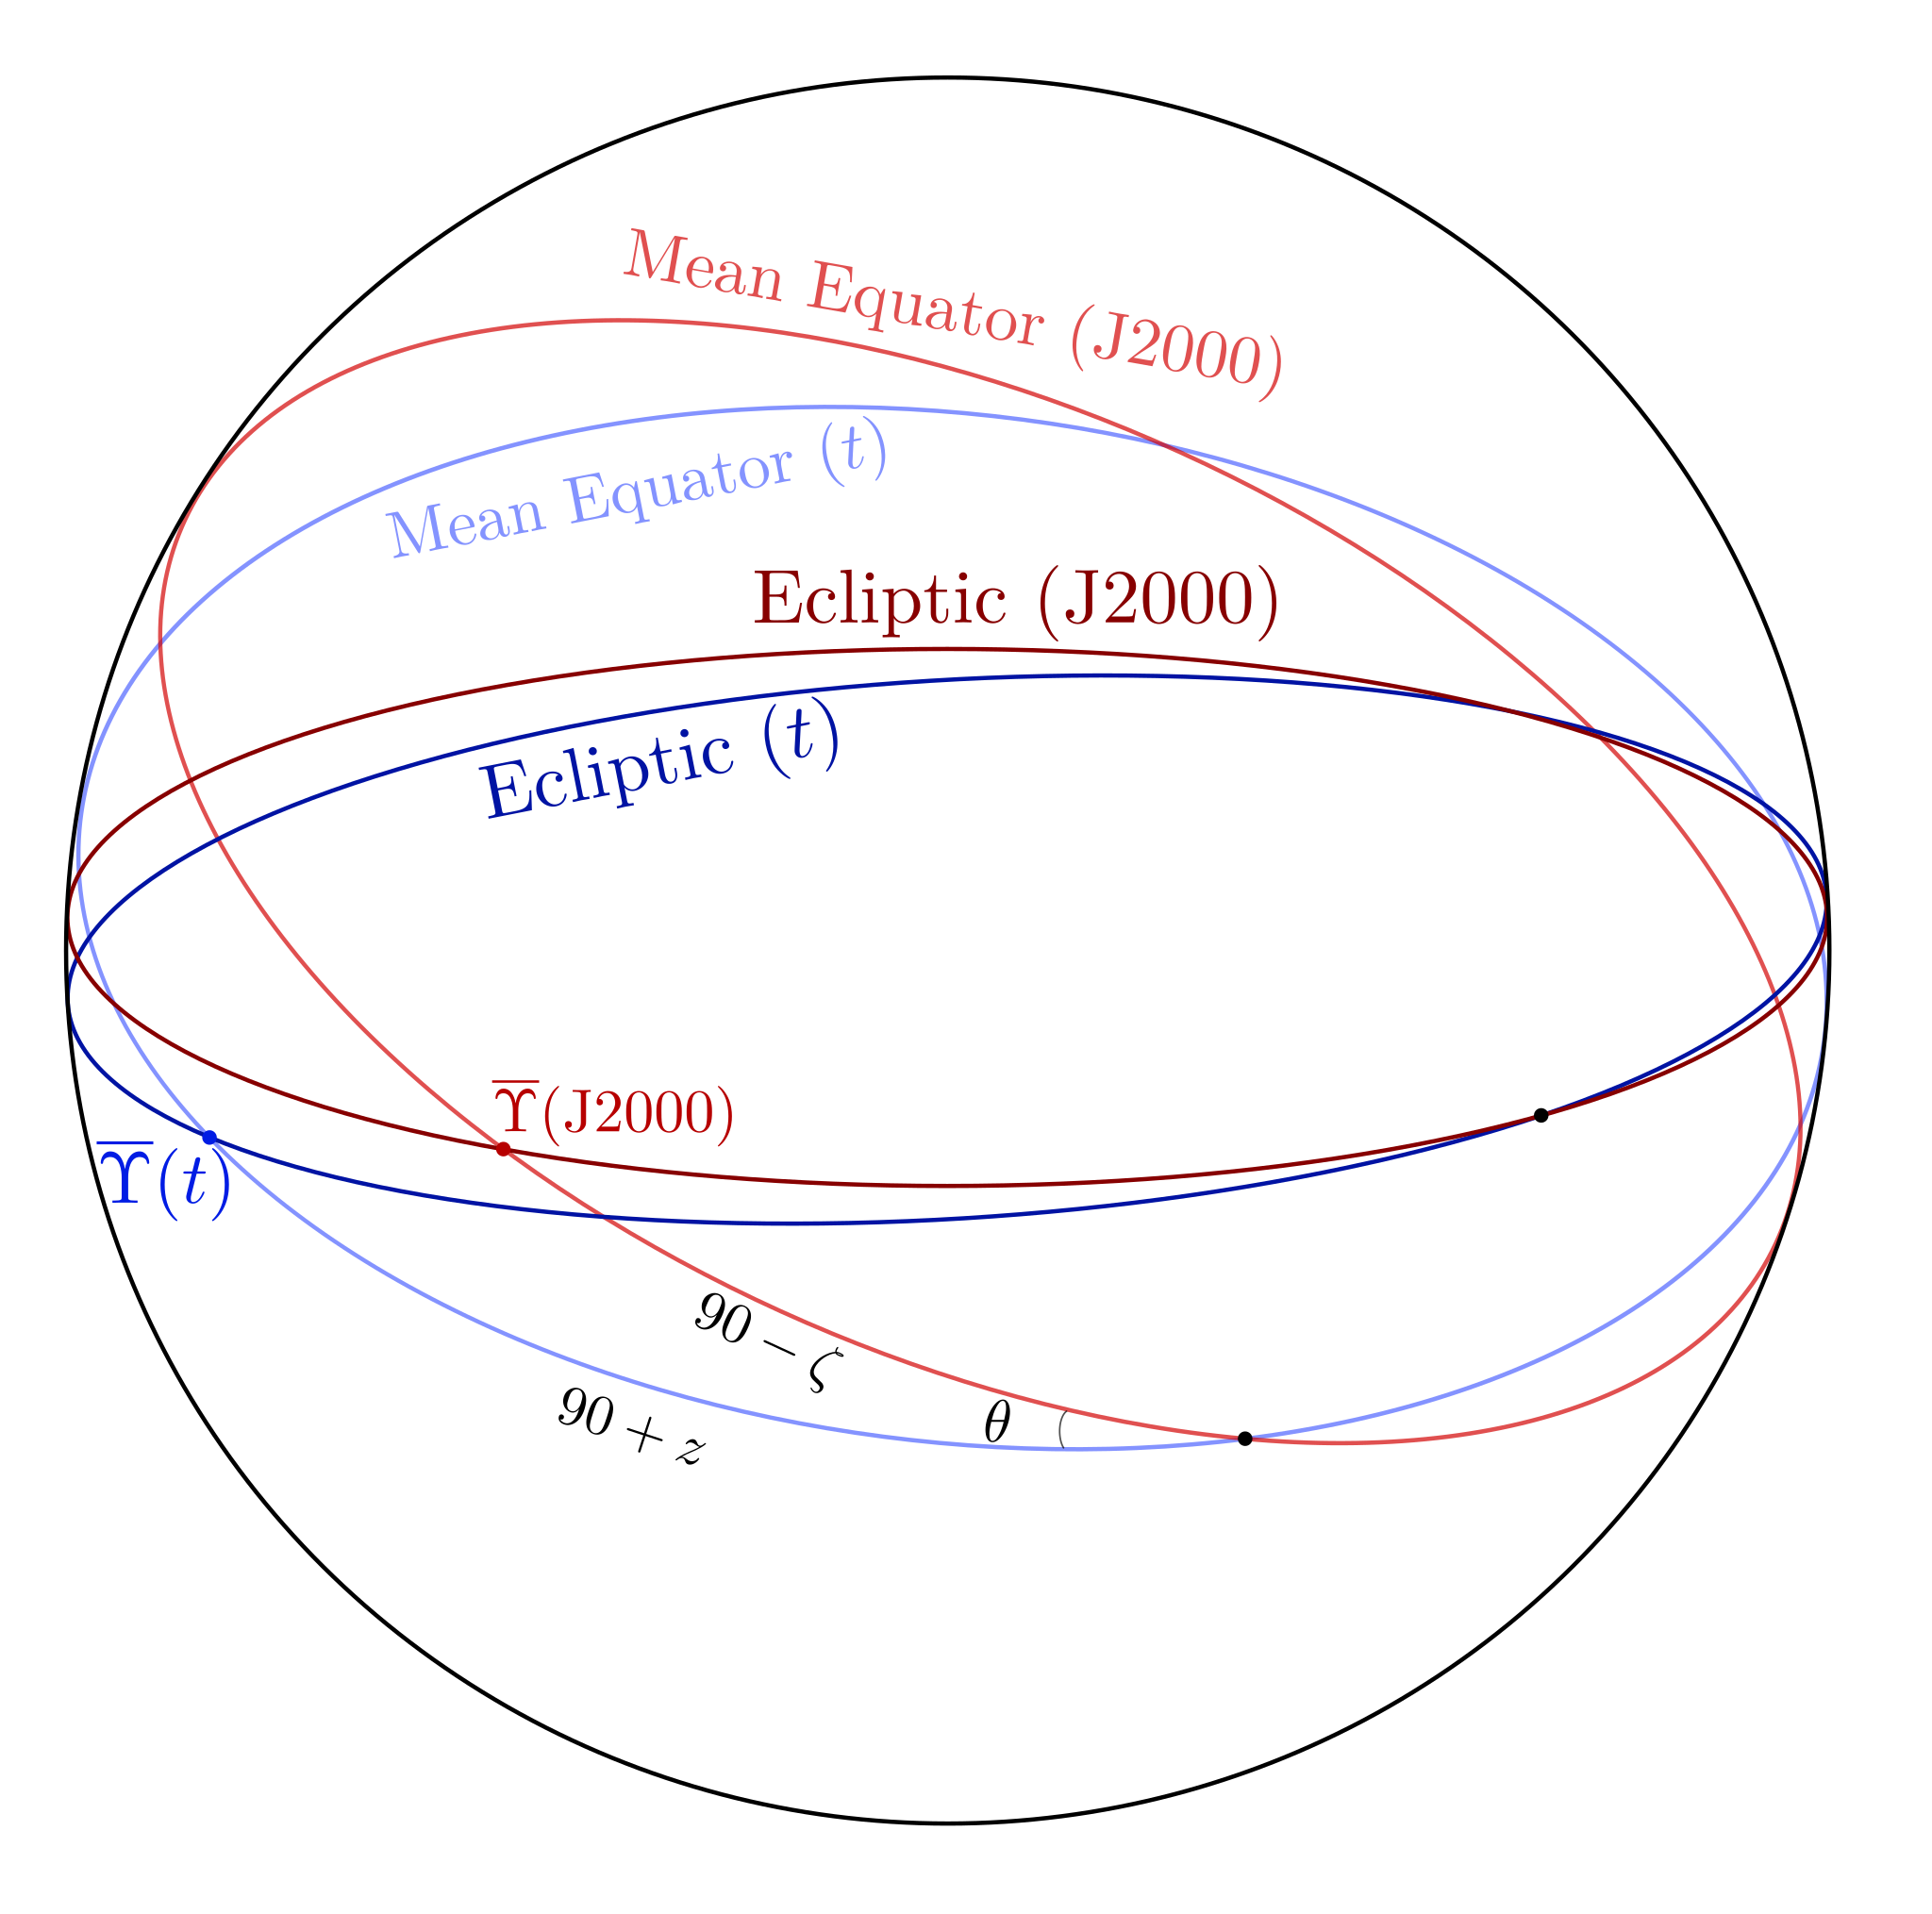
\includegraphics[width=\textwidth]{Images/ecliptic_equator.pdf}
    \caption{Celestial sphere showing the ecliptic and the equator of both the epoch J2000 and the current epoch $t$. Dark colors represent the ecliptic while light colors represent the equator. On the other hand, red colors represents the the J2000 epoch and blue colors represents the current epoch $t$.}
    \label{fig:precession_matrix}
  \end{minipage}
  \hfill
  \begin{minipage}[t]{0.45\textwidth}
    \centering
    \includegraphics[width=\textwidth]{Images/nutation_matrix.pdf}
    \caption{True equator and mean equator, and true equinox ($\Upsilon'$) and mean equinox ($\Upsilon$) at a given epoch $t$ together with the ecliptic at that time.}
    \label{fig:nutation_matrix}
  \end{minipage}
\end{figure}
The reader may wonder why we have used the notation $90-z$ and $90-\zeta$ instead of $z$ and $\zeta$ (for example) for the angles in question. The reason is related to the precise definition of these angles from the pole of the celestial sphere rather than from where we have defined them, but we will not elaborate on this point here. Nonetheless, we have chosen this notation to maintain consistency with related articles.

The nutation perturbations are driven out by the nutation matrix $\mathbf{N}$. This matrix transforms the coordinates of the mean equator and equinox at epoch $t$ to those of the true equator and equinox at the same epoch, respectively. Hence, from figure \cref{fig:nutation_matrix} we can see that the nutation matrix is given by:
\begin{equation}
  \mathbf{N}=\vf{R}_x(-\varepsilon-\Delta \varepsilon)\vf{R}_z(-\Delta \psi)\vf{R}_x(\varepsilon)
\end{equation}
\subsection{Orbital elements}
\subsubsection{Orbital elements from position and velocity}
\begin{definition}
  Consider a satellite orbiting the Earth. The \emph{orbital plane} is the plane that contains the orbit of the satellite. The \emph{line of nodes} of intersection between the orbital plane and the equator. Finally, the \emph{ascending node} is the point on the line of nodes and the orbit of the satellite where the satellite crosses the equatorial plane from south to north.
\end{definition}
\begin{definition}[Orbital elements]
  The \emph{orbital elements} of a satellite are five independent quantities that completely determine its orbit. If moreover the exact position of the satellite on the orbit is wanted, a sixth quantity is needed. The first five orbital elements are:
  \begin{enumerate}
    \item The \emph{semi-major axis} $a$ of the orbit.
    \item The \emph{eccentricity} $e$ of the orbit.
    \item The \emph{inclination} $i$ is the angle between the equatorial plane and the orbital plane.
    \item The \emph{longitude of the ascending node} $\Omega$ is the angle between the vernal equinox and the ascending node.
    \item The \emph{argument of perigee} $\omega$ is the angle between the ascending node and the periapsis.
  \end{enumerate}
  The sixth quantity is the \emph{true anomaly} $\nu$ which is the angle between the periapsis and the position of the satellite on the orbit.
\end{definition}
The elements $a$, $e$ and $i$ are always well-defined. However, the elements $\Omega$, $\nu$ are not well-defined in the case of $e=0$ because there is no periapsis, because all the points lie at the same distance from the center of the Earth.
Note that $i\in [0,\pi/2]$ and by convention we will impose the angles  $\Omega$, $\omega$, $\nu$ to be in  $[0,2\pi)$
\begin{figure}[ht]
  \centering
  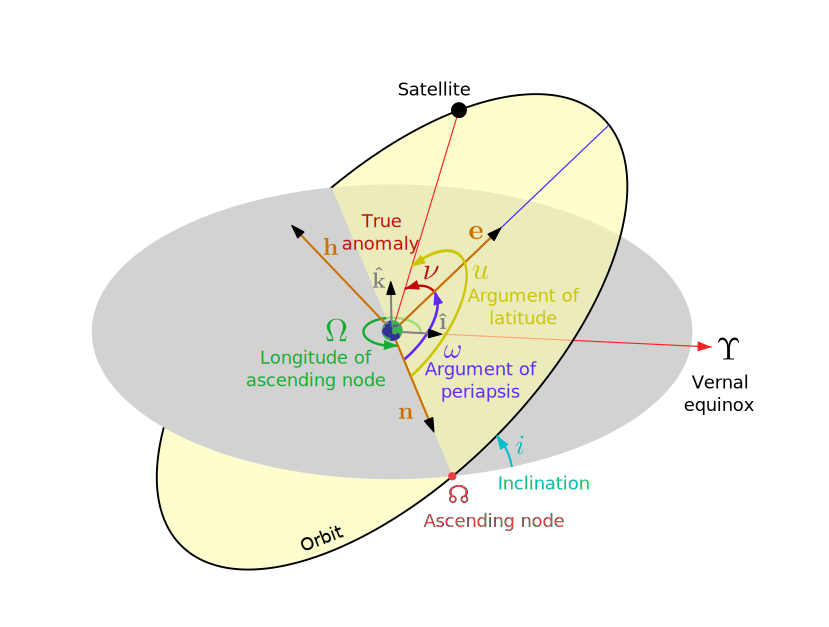
\includegraphics[width=0.8\textwidth]{Images/orbital_elements.pdf}
  \caption{Orbital elements of a satellite.}
  \label{fig:orbital_elements}
\end{figure}
In order to properly define these elements in terms of the position $\vf{r}$ and the velocity $\dot{\vf{r}}$ of the satellite, we need to introduce the basis $(\vf{p}, \vf{q}, \vf{w})$ linked to the orbit.
\begin{definition}[Perifocal coordinate system]
  Consider the orbit of a satellite. We define its associated \emph{perifocal coordinate system} $(\vf{p}, \vf{q}, \vf{w})$ as follows. The center is on the Earth's center of mass. The unit vectors $\vf{p}$ and $\vf{q}$ lie on the orbital plane and are such that $\vf{p}$ points towards the periapsis, that is $\vf{p}:=\vf{B}/B$. The unit vector $\vf{w}$ is defined as $\vf{w}:=\vf{h}/h$ and $\vf{q}:=\vf{w}\times\vf{p}$.
\end{definition}

\begin{theorem}
  Consider a satellite orbiting the Earth at position $\vf{r}$ and velocity $\dot{\vf{r}}$ from the Earth-fixed frame. The orbital elements of the satellite are given by:
  \begin{align*}
    a      & = {\left(\frac{2}{r}-\frac{v^2}{\mu}\right)}^{-1} & e      & = \sqrt{1-\frac{p}{a}}                                   & i   & = \arccos\left(\frac{h_z}{h}\right)          \\
    \Omega & = \arctan\left(\frac{h_x}{-h_y}\right)\mod 2\pi   & \omega & =\arctan\left(\frac{B_zh}{h_xB_y-h_yB_x}\right)\mod 2\pi & \nu & =\arccos\left(\frac{p-r}{re}\right)\mod 2\pi
  \end{align*}
  where $\vf{h}=(h_x,h_y,h_z)$ and $\vf{B}= (B_x,B_y,B_z)$.
\end{theorem}
\begin{proof}
  First note that we can know $\vf{h}$ and $p$ from $\vf{h}=\vf{r}\times \dot{\vf{r}}$ and $p=h^2/\mu$. Moreover $\vf{B}=\dot{\vf{r}}\times \vf{h}-\frac{\mu}{r}\vf{r}$ form \cref{eq:rdottimesh}. The semi-major axis $a$ is given in \cref{eq:visviva} and the eccentricity formula follows from \cref{eq:semi-major_axis}. Isolating $\nu$ from the equation of the ellipse (\cref{eq:r_conic}) we can get the true anomaly. Moreover, one can note (looking at \cref{fig:orbital_elements}) that the matrix transformation from the perifocal frame to the Earth-fixed frame is given by:
  \begin{equation}
    \vf{A}=\vf{R}_z(-\Omega)\vf{R}_x(-i)\vf{R}_z(-\omega)
  \end{equation}
  Now, from linear algebra we know that $(\vf{p}, \vf{q}, \vf{w})$ are just the column vectors of $\vf{A}$. From here, computing $\vf{A}$ we get that:
  \begin{equation}
    \vf{A}= \begin{pmatrix}
      \cos(\omega)\cos(\Omega)-\sin(\omega)\sin(\Omega)\cos(i) & -\sin(\omega)\cos(\Omega)-\cos(\omega)\sin(\Omega)\cos(i) & \sin(\Omega)\sin(i)  \\
      \cos(\omega)\sin(\Omega)+\sin(\omega)\cos(\Omega)\cos(i) & -\sin(\omega)\sin(\Omega)+\cos(\omega)\cos(\Omega)\cos(i) & -\cos(\Omega)\sin(i) \\
      \sin(\omega)\sin(i)                                      & \cos(\omega)\sin(i)                                       & \cos(i)
    \end{pmatrix}
  \end{equation}
  From the definition we can get $\vf{p}$ and $\vf{w}$ by:
  \begin{equation}
    \vf{p}=\begin{pmatrix}
      B_x/B \\
      B_y/B \\
      B_z/B
    \end{pmatrix}\qquad
    \vf{w}=\begin{pmatrix}
      h_x/h \\
      h_y/h \\
      h_z/h
    \end{pmatrix}
  \end{equation}
  From here and looking at the third column of $\vf{A}$ we deduce the expressions for $i$ and $\Omega$. Now, if $\vf{q}=(q_x, q_y, q_z)$, we have that $q_z=w_x p_y-w_y p_x=\frac{h_x B_y-h_yB_x}{hB}$ and so:
  \begin{equation}
    \frac{B_z/B}{(h_x B_y-h_yB_x)/hB}=\tan(\omega)\implies \omega =\arctan\left(\frac{B_zh}{h_xB_y-h_yB_x}\right)
  \end{equation}
\end{proof}
Està relament be????????????????????????? Pensar en que els TLE estan referits respecte el j2000 o no?????
\subsubsection{TLE sets and determining position and velocity from orbital elements}
The positions of satellites at each instant of time
\end{document}